\documentclass[a4paper,12pt]{article}
% Packages
\usepackage{geometry}
\geometry{left=2.54cm, right=2.54cm, top=2.54cm, bottom=2.54cm}
\usepackage{enumitem}
\usepackage{titlesec}
\usepackage{hyperref}
\usepackage{graphicx}
\usepackage{setspace}
\setstretch{1.2}

% Set up fonts
\usepackage{helvet}
\renewcommand{\familydefault}{\sfdefault}

% Set up section formatting
\titleformat{\section}{\large\bfseries}{}{0em}{}[\titlerule]
\titleformat{\subsection}{\bfseries}{}{0em}{}

% Set up itemize formatting
\setlist[itemize]{noitemsep, topsep=0pt}
\begin{document}

% Header
\begin{center}
    {\LARGE \textbf{Viet Anh Dong}} \\
    \vspace{1mm}
    \href{mailto:dongvietanh@gmail.com}{Email: dongvietanh@gmail.com} \\
    \href{https://github.com/yourusername}{Github: github.com/yourusername} \\
    \href{https://www.linkedin.com/in/vietanhdong}{Linkedln Profile: linkedin.com/in/vietanhdong}\\
    Address: St Lucia, Queensland, Australia, 4067 \\
\end{center}

% Career Development and Objective
\section*{Career Development and Objective}
A forestry specialist who has strong experience in forestry and data analysis. \newline
Currently, I am looking for a position that allows me to utilize my skills in data analysis to solve real-world problems.

\begin{figure}[ht]
    \centering
    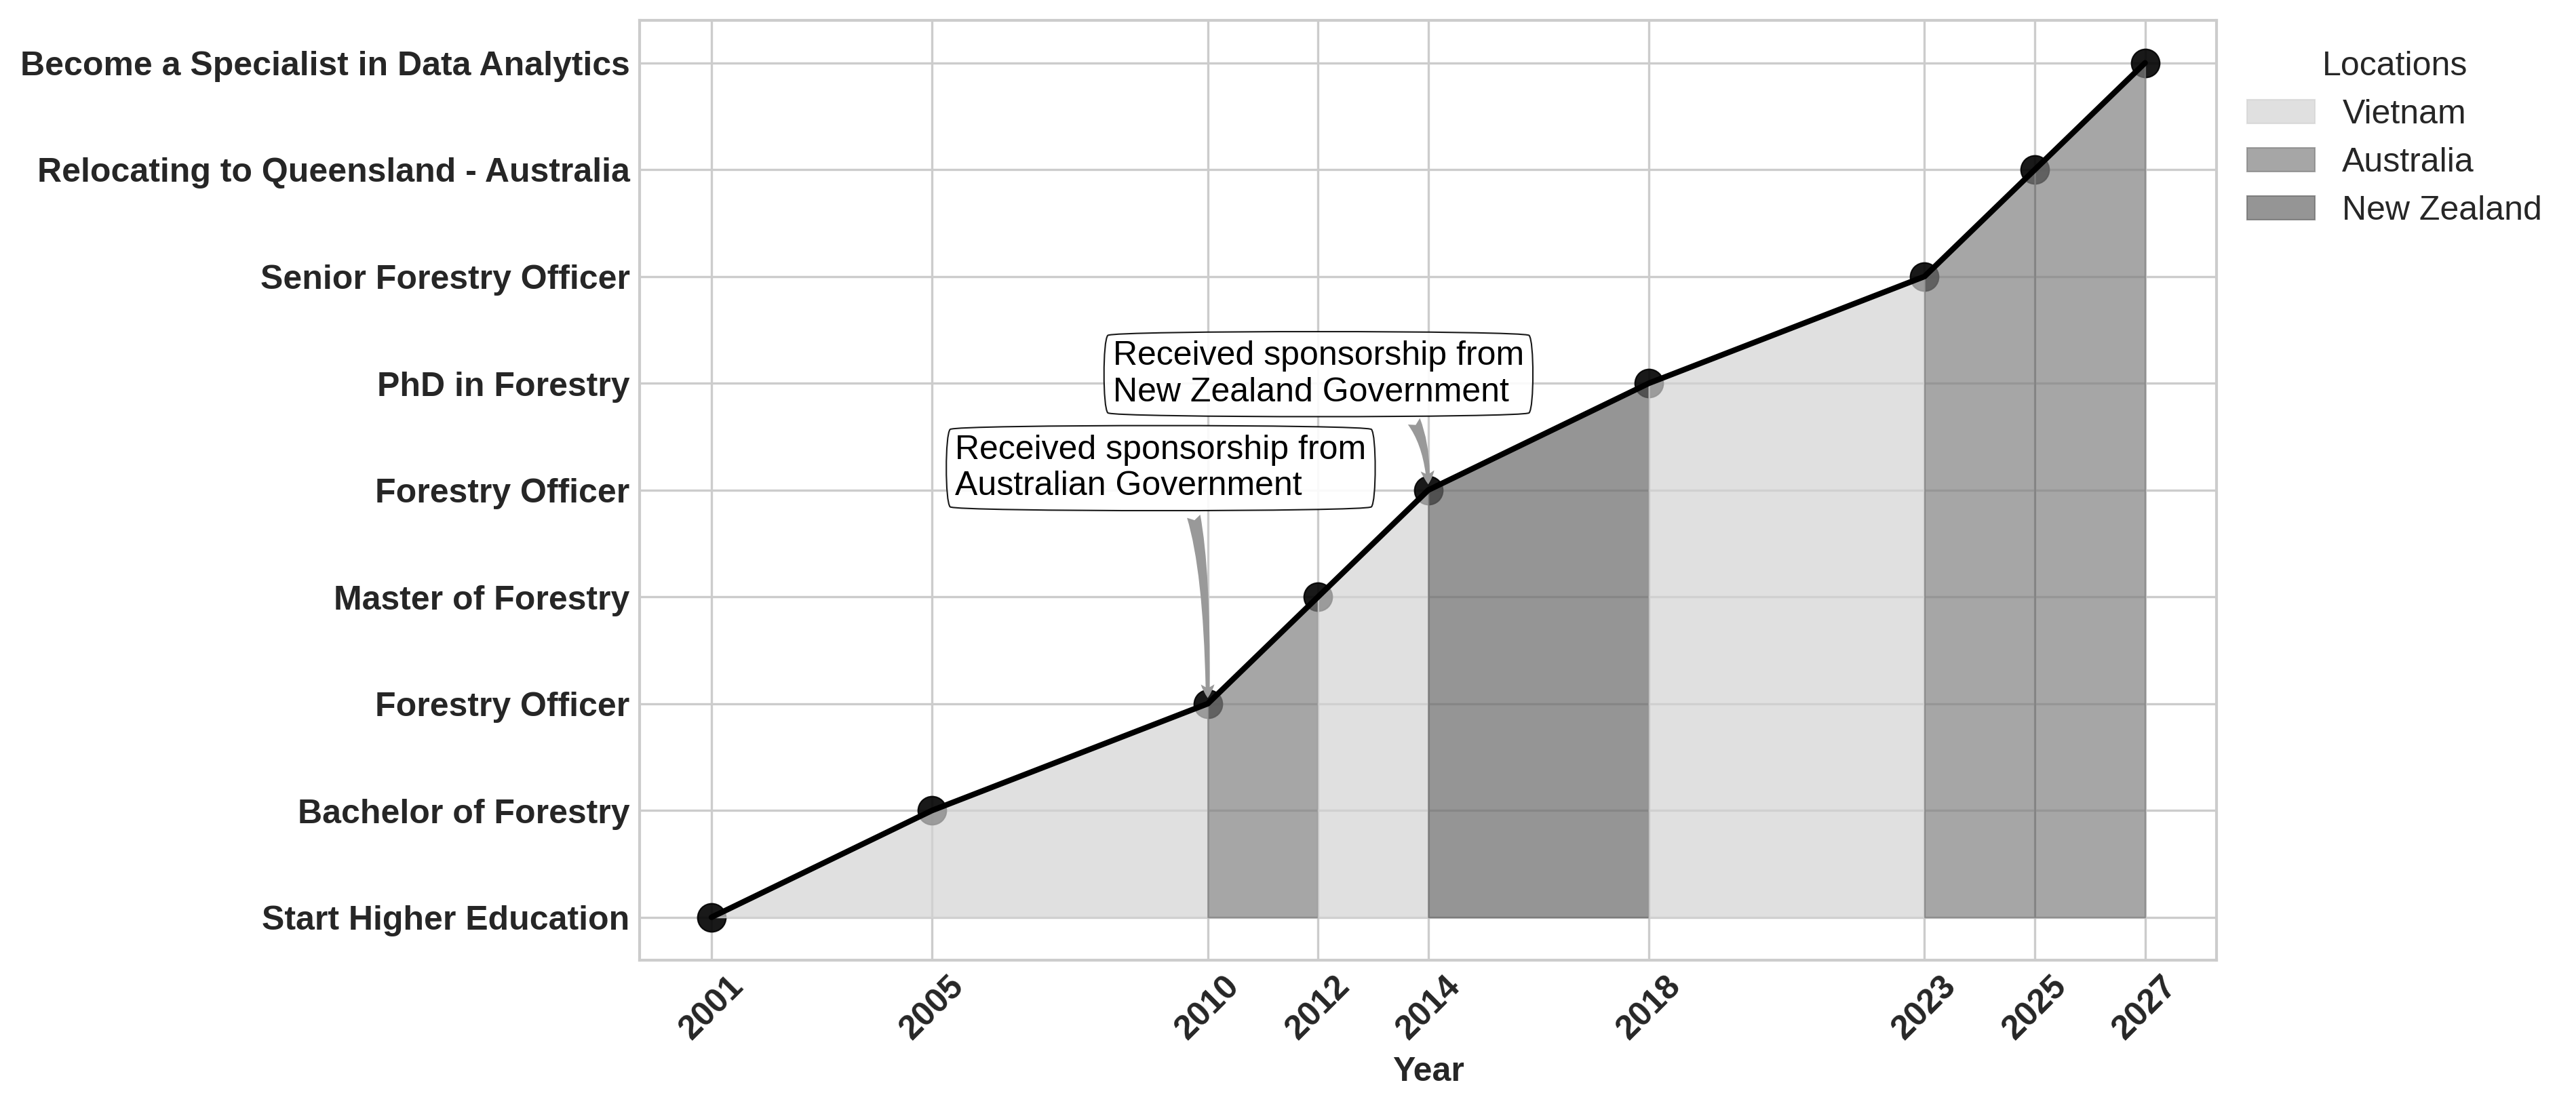
\includegraphics[width=\textwidth]{/mnt/d/Viet-Anh-Dong-resume/professional.png}
    \caption{Professional Timeline}
    \label{fig:your_image}
\end{figure}

% Education
\section*{Education}
University of Canterbury, Christchurch, New Zealand \newline
\textbf{PhD in Forestry} \hfill Graduation Year: 2018 \newline

\par % start a new paragraph
\noindent
Australian National University, Canberra, Australia \newline
\textbf{Master of Forestry} \hfill Graduation Year: 2012 \newline
\textbf{Graduate Diploma in Environmental and Management} \hfill Graduation Year: 2012 \newline

\par % start a new paragraph
\noindent
Thai Nguyen University of Agriculture and Forestry, Thai Nguyen, Vietnam \newline
\textbf{Bachelor of Forestry} \hfill Graduation Year: 2006

% Experience
\section*{Professional Experience}

\vspace{1em} % add vertical space
\noindent
\textbf{Relocating to Australia and Self-training} \hfill October 2023 - Present \newline
Relocating to Australia as a family of four with two boys and a commiment to self-training gave me opotunities to: \newline

\vspace{-1.5em} % reduce vertical space
\begin{itemize}
    \item Leverage self-training to develop new skills in data analysis.
    \item Navigating the challenges of relocating to a new country and integrating into a new culture strengthening my ability to adapt to new environments and stituations.
    \item Developed a project on [Brief Description of Project], which can be found at \href{https://github.com/yourusername/project}{github.com/yourusername/project}
    \item Earned certifications in [Relevant Certifications]
    \item Participated in [Relevant Workshops, Seminars, or Conferences]
\end{itemize}

\vspace{1em} % add vertical space
\noindent
\textbf{Academic Experience} \hfill November 2014 -- March 2018 \newline
Spending four years as a PhD candidate provided me with:. \newline
\vspace{-1.5em} % reduce vertical space
\begin{itemize}
    \item Advanced research skills
    \item Critical analytical abilities
    \item Practical experience managing complex projects
\end{itemize}

\vspace{1em} % add vertical space
\noindent
\textbf{Forestry Officer} \hfill May 2006 -- August 2022 \newline
The combination of hand-on filed experience and professional training at a prestigious Australian institution, Australia Nationa University, has provided me with excellent skills in management, including:\newline

\vspace{-1.5em} % reduce vertical space
\begin{itemize}
    \item Integrate research, field data, and strategic planning to develop and implement sustainable forestry practices.
    \item Enhance my ability to lead and collaborate with stakeholders to achieve common goals.
    \item Cultivate strong problem solving and critical thinking skills.
    \item Use data analytics and research methodologies to inform decision-making and drive continuous improvement.
\end{itemize}

% Projects
\section*{Projects}
\noindent
\textbf{Resume} \newline
\vspace{-1.5em} % reduce vertical space
\begin{itemize}
    \item The repository contains my lastest resumme showcase my skills and experience
    \item Technologies used: Latex, Python, Vscode, Git, matplotlib
    \item Repository link: \href{https://github.com/yourusername/project}{github.com/yourusername/project} 
\end{itemize}
\noindent
\textbf{Loan Status Prediction}  \newline
\vspace{-1.5em} % reduce vertical space
\begin{itemize}
    \item Analyse and predict loan status and creadit score of potential clients use neural networks with two outputs.
    \item Technologies used: Python, Jupyter Notebook, Git, matplotlib, tensorflow, tensorboard, scikit-learn, keras.
    \item Repository link: \href{https://github.com/ant-analytics/loan-status.git}{github.com/ant-analytics/loan-status}
\end{itemize}

% Skills
\section*{Technical Skills}
\begin{itemize}
    \item \textbf{Programming:} R, Python
    \item \textbf{Development, Data Science and GIS Tools:} Rstudio, Jupyter Notebook, Anaconda, Git, Vscode, QGIS
    \item \textbf{Analytical and Statistical skills:} hypothesis testing, regression and classification models, machine learning, neural networks, data visualization.
\end{itemize}

\section*{Soft Skills}
\begin{itemize}
    \item \textbf{Soft Skills:} Teamwork, Self-Development, Research and Development, Highly Adaptive to New Environment
    \item \textbf{Soft Skills:} Teamwork, Self-Development, Research and Development, Highly Adaptive to New Environment
\end{itemize}

% Certifications
\section*{Certifications}
\noindent
\textbf{Stanford University \& DeepLearning.AI} \newline
\textit{Machine Learning Specialization} \hfill \textit{April 2023} \newline
Course Certificates Completed:
\begin{itemize}
    \item Supervised Machine Learning: Regression and Classification
    \item Advanced Learning Algorithms
    \item Unsupervised Learning, Recommender, Reinforcement Learning
\end{itemize}

% Additional Information
\section*{Additional Information}
\begin{itemize}
    \item \textbf{Australian Work Right:} Unlimited work and study entitlements
    \item \textbf{Driver's License:} Class CA (Automatic Car) - Type: O (Open)
    \item \textbf{Police and Health Check:} Available upon request
    \item \textbf{References:} Available upon request
    \item \textbf{Australia, New Zealand qualifcations and online training ceritifcates} Available upon request
    \item \textbf{Languages:} Vietnamese (Native), English (Fluent)
    \item \textbf{Interests:} Hiking, Photography, Reading
\end{itemize}

\end{document}